% 中文节标题：实验
% 中文：阻止实验内容回漂到方法节。
\FloatBarrier
\section{Experiments}
\label{sec:experiments}

% 中文：我们评测统一世界坐标中的多镜头多人体重建，重点分析大视角变化、对齐与状态传播、人物关联、镜头检测和效率。
We evaluate multi-shot multi-person reconstruction in a common world frame,
with emphasis on large viewpoint changes, alignment and state propagation,
person association, transition detection, and efficiency.

% 中文：在4.1实验设置之前引入核心定性结果。
\begin{figure*}[t]
  \centering
  % 从完整可编辑七方法图中无损裁取正文关键方法列；完整版本见附录。
  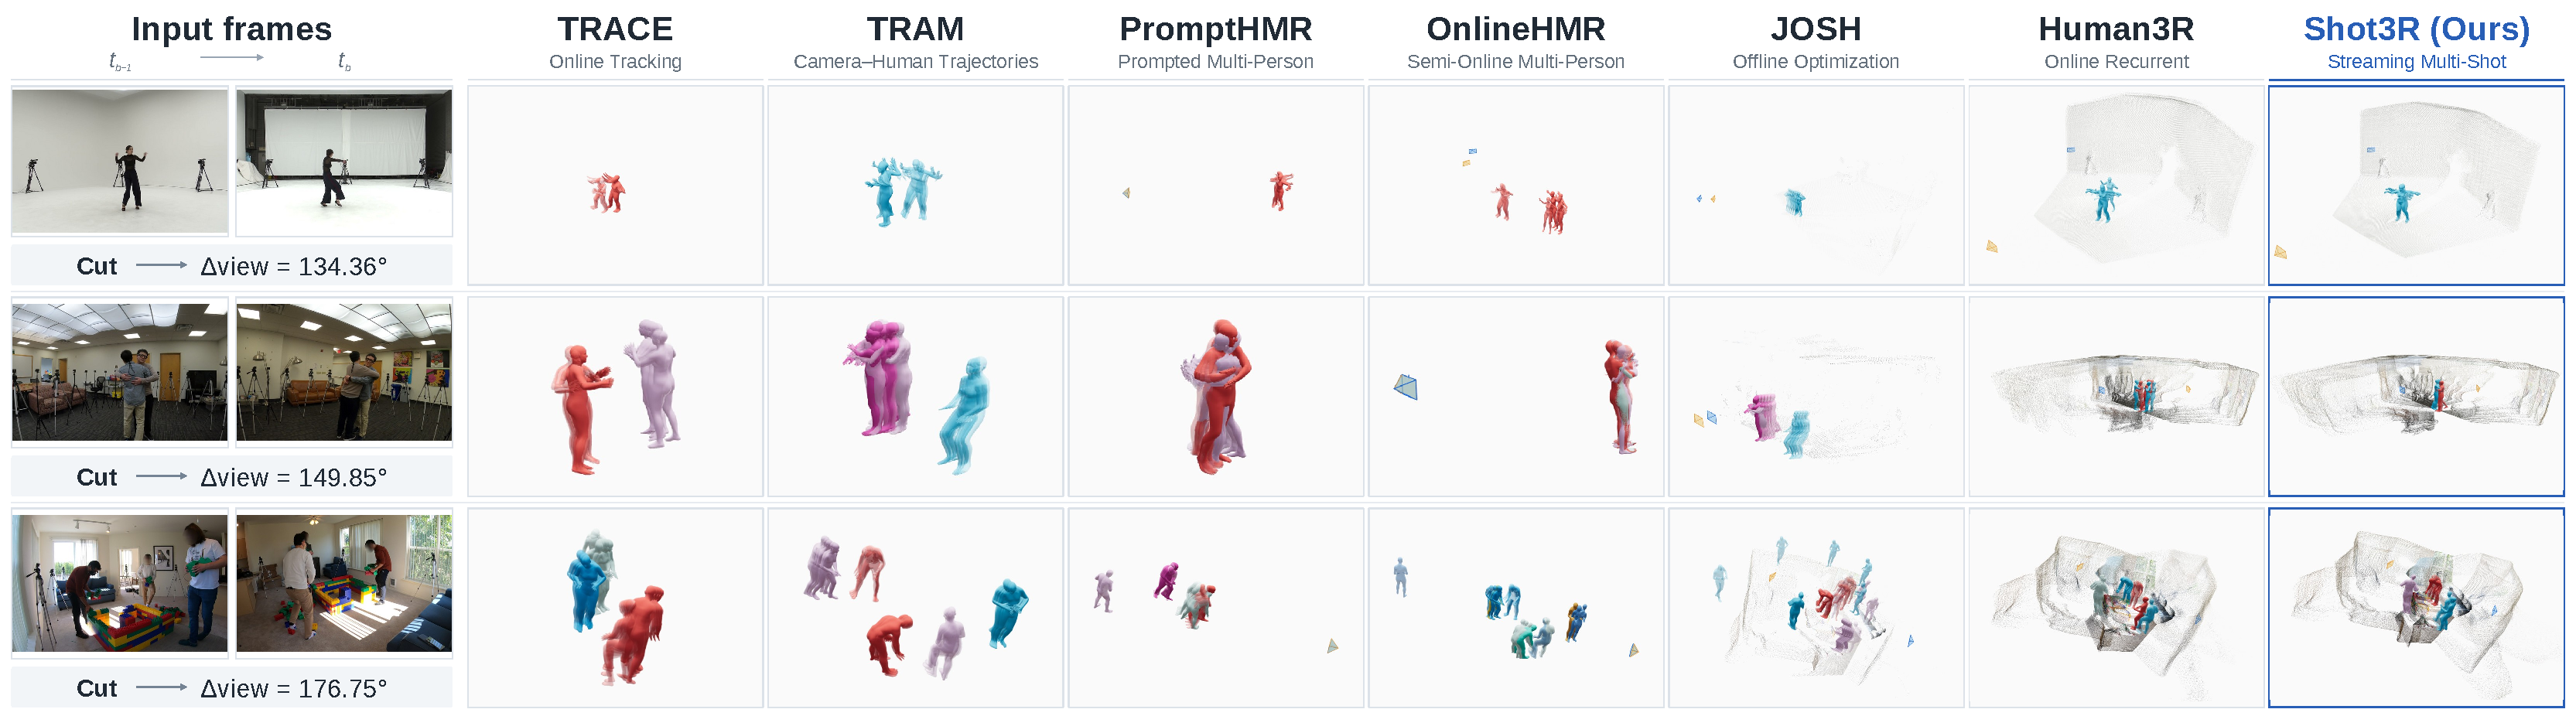
\includegraphics[height=0.415\textwidth,trim=0pt 0pt 1315pt 0pt,clip]{figures/Shot3R_qualitative_comparison.pdf}\hspace{-1.2mm}%
  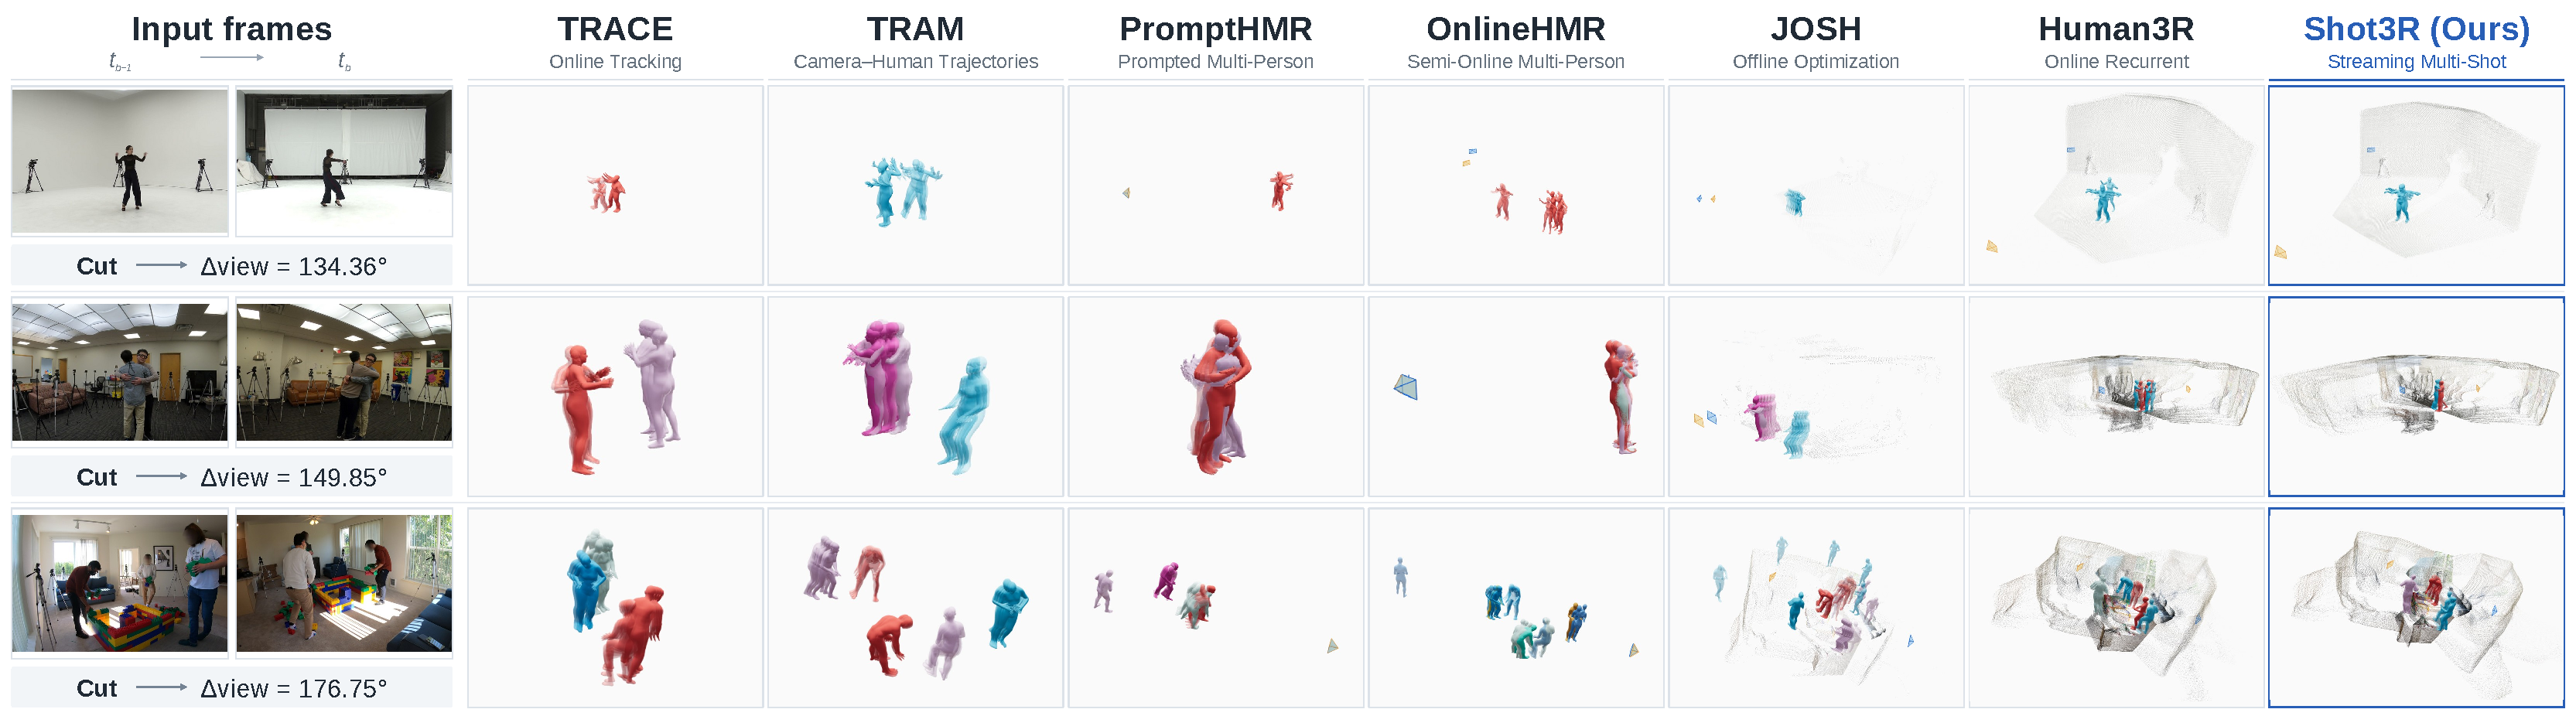
\includegraphics[height=0.415\textwidth,trim=845pt 0pt 560pt 0pt,clip]{figures/Shot3R_qualitative_comparison.pdf}\hspace{-1.2mm}%
  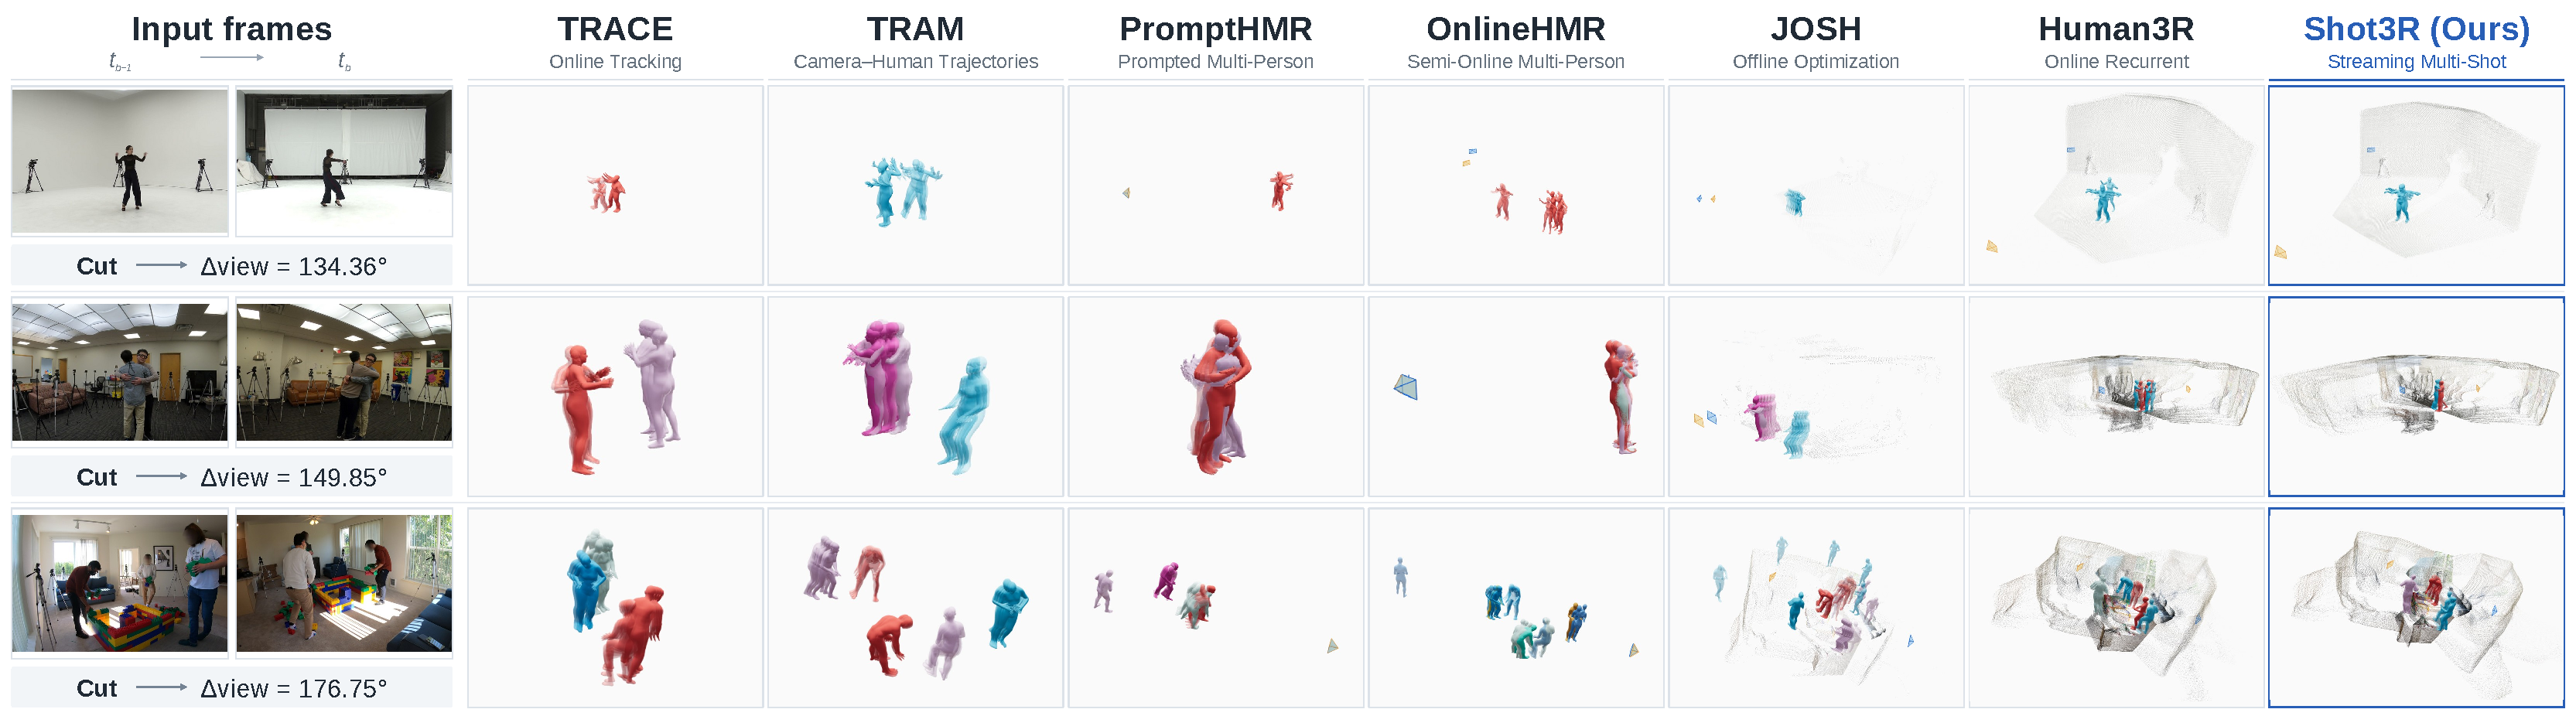
\includegraphics[height=0.415\textwidth,trim=1034pt 0pt 374pt 0pt,clip]{figures/Shot3R_qualitative_comparison.pdf}\hspace{-1.2mm}%
  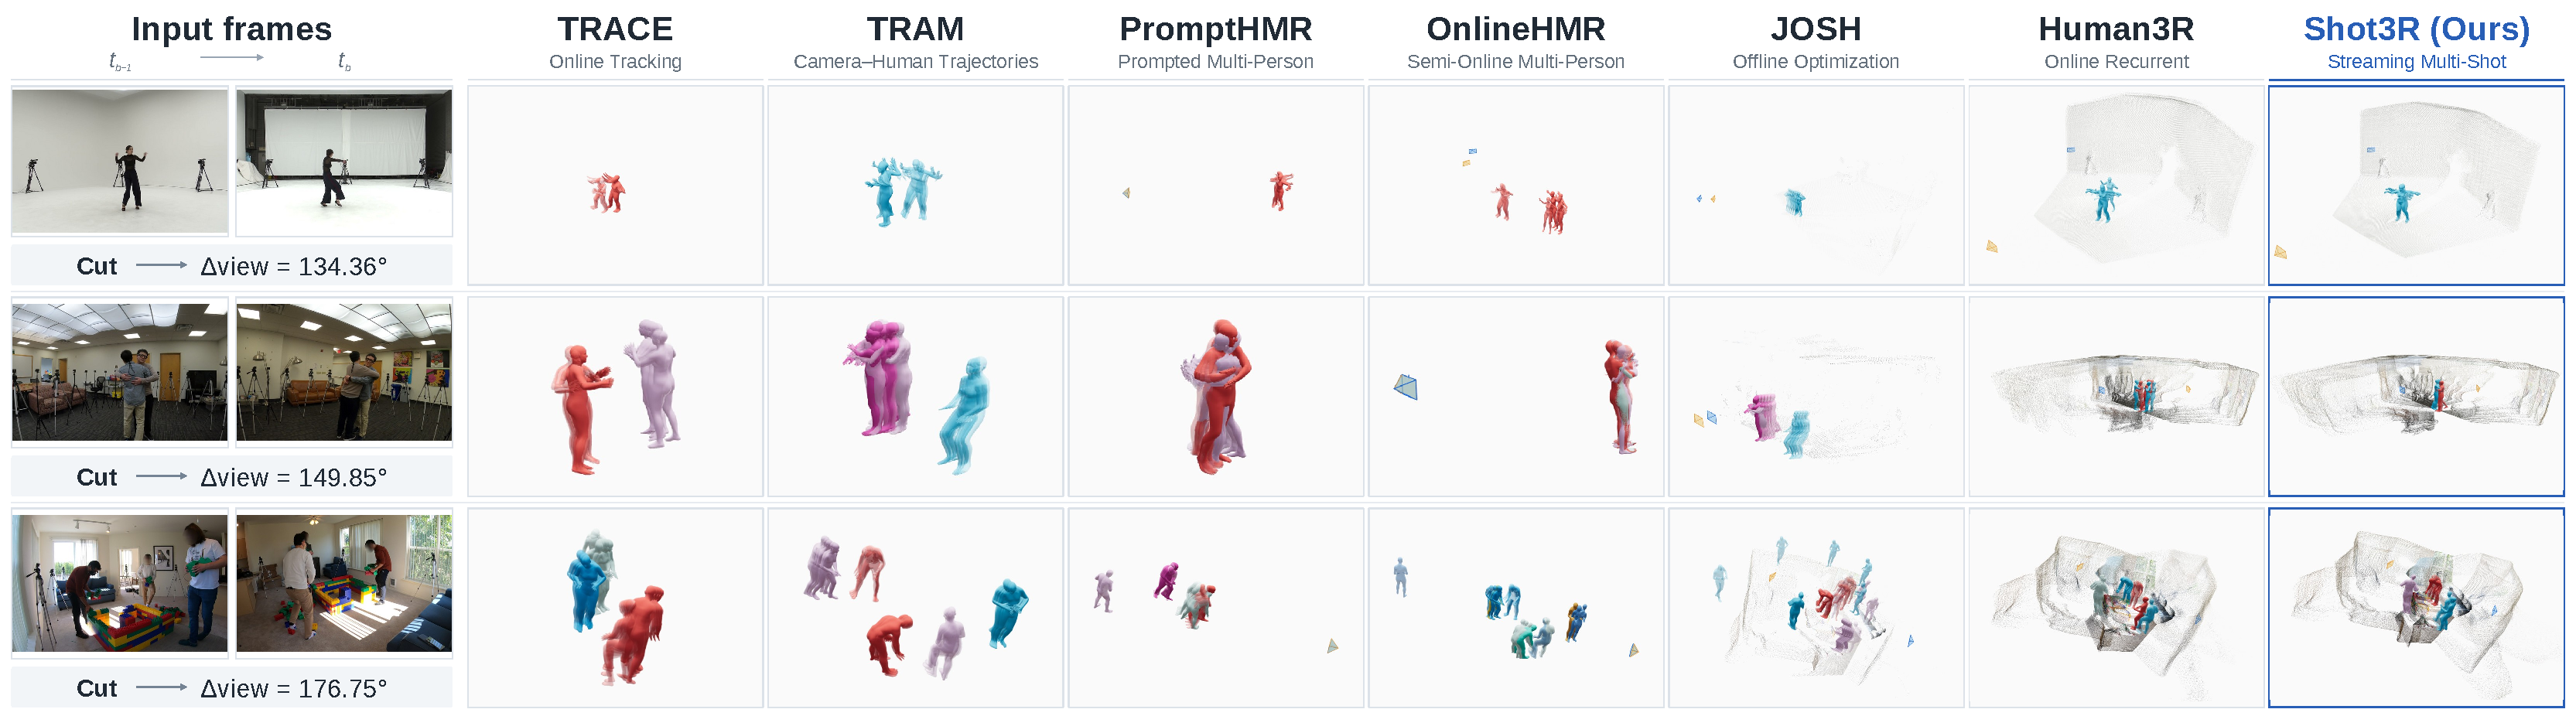
\includegraphics[height=0.415\textwidth,trim=1220pt 0pt 188pt 0pt,clip]{figures/Shot3R_qualitative_comparison.pdf}\hspace{-1.2mm}%
  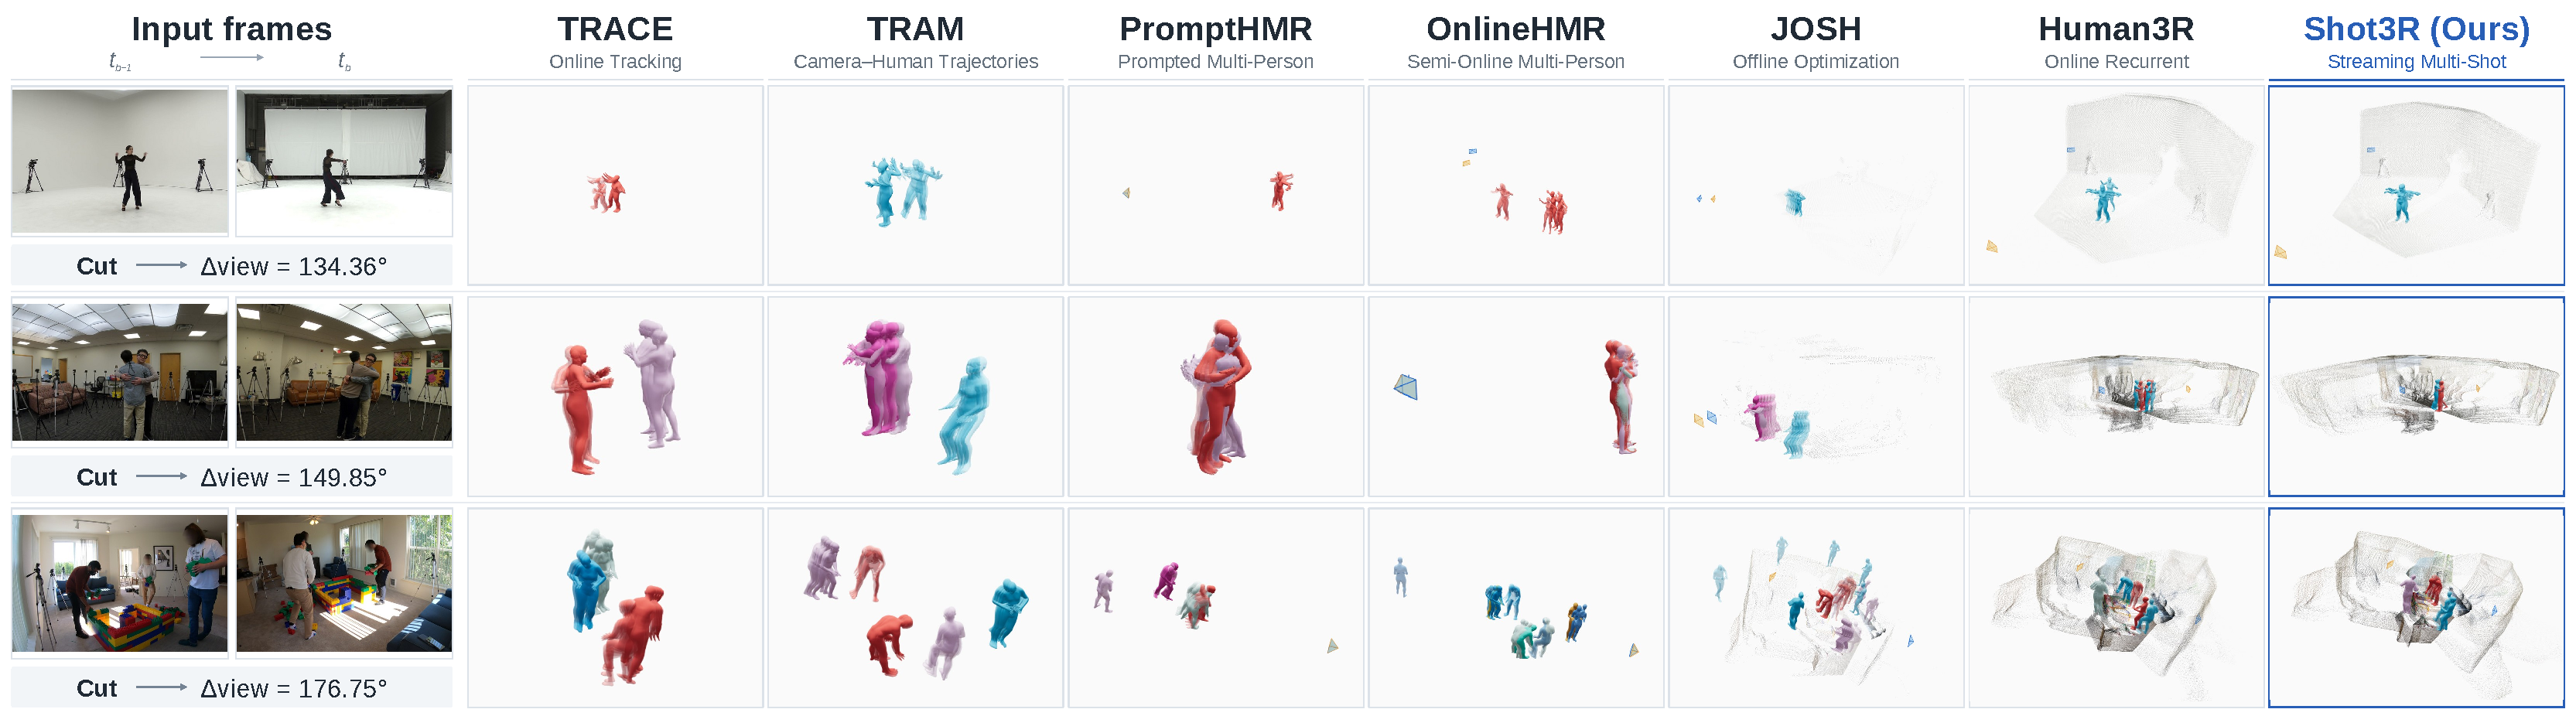
\includegraphics[height=0.415\textwidth,trim=1407pt 0pt 0pt 0pt,clip]{figures/Shot3R_qualitative_comparison.pdf}
  % 中文图注：跨镜头切换的关键定性比较。每一行首先展示切换前后的输入，随后是半在线、离线、在线递归基线与本文结果。
  % 三个视角变化从上到下为134.36、149.85和176.75度。Shot3R维持更连贯的相机—人体布局；各方法可用的场景输出一并显示。
  \caption{\textbf{Key qualitative comparisons across shot transitions.}
  Inputs before and after each transition are followed by OnlineHMR, JOSH,
  \humanthree{}, and \method{}. Viewpoint changes are $134.36^\circ$,
  $149.85^\circ$, and $176.75^\circ$ from top to bottom. \method{} maintains a
  more coherent camera--human layout; scene geometry is shown where available.
  The complete seven-method view is in Appendix~\ref{app:qualitative-full}.}
  \label{fig:qualitative-comparison}
\end{figure*}


% 中文小节标题：实验设置
\subsection{Experimental Setup}

% 中文段落标题：对比方法。
% 中文：Human3R是主要受控基线，两种方法接收相同的顺序RGB输入并使用相同评测；区别在于Human3R持续传播状态，而Shot3R在检测到切换时完成对齐并重新初始化后续状态。
% 我们还运行OnlineHMR、TRACE、PromptHMR、JOSH和TRAM的公开实现，并按其时间访问方式进行比较。
\paragraph{Baselines.}
\humanthree{} is the primary controlled baseline: both methods receive the
same ordered RGB frames and evaluation, but \humanthree{} propagates state
uninterruptedly whereas \method{} aligns the shots and propagates a reinitialized
state through the new shot. We also run the official implementations of OnlineHMR, TRACE, PromptHMR,
JOSH, and TRAM~\citep{zhao2026onlinehmr,sun2023trace,wang2025prompthmr,liu2026josh,wang2024tram}.
Table~\ref{tab:multi-person} groups them by temporal access and marks explicit
transition handling; preprocessing and output scope are reported in
Appendix~\ref{app:protocol}. OnlineHMR combines semi-online person tracking
with a separate global-camera backend, PromptHMR and JOSH process the complete
video, and TRAM is included in the standardized full-system timing study.
HumanMM and Multi-THuMBS lack the complete
public code, weights, and configurations needed for our fixed inputs; their
task scope is summarized in Table~\ref{tab:supp-baseline-scope} rather
than mixing results from different protocols.

% 中文段落标题：数据集与评价指标。
% 中文：三个主协议将EgoBody、EgoHumans和Harmony4D的同步采集转换为依次出现的两段单目RGB流，共129、90和88个固定样例；模型始终逐帧接收输入。
\paragraph{Datasets and metrics.}
We convert synchronized EgoBody, EgoHumans, and Harmony4D captures
~\citep{zhang2022egobody,khirodkar2023egohumans,khirodkar2024harmony4d} into
two sequential monocular shots, yielding 129, 90, and 88 fixed cases,
respectively. The model receives one temporally ordered frame at a time. The
datasets provide complementary evidence: EgoBody supports controlled mechanism
ablations, EgoHumans emphasizes large viewpoint changes and recurrent-state
carry-over, and Harmony4D evaluates person association and repeated transitions.

% 中文：W-MPJPE用最早有效观测确定并固定Sim(3)，对跨镜头轨迹偏移敏感；WA-MPJPE使用全部有效观测进行Sim(3)对齐。
% 相机误差在EgoBody/Harmony4D上为ATE-Sim3，在EgoHumans上为ATE-SE3；IDF1评估身份连续性，Coverage防止缺失预测从条件人体误差中消失。
W-MPJPE (W) fixes a Sim(3) alignment from the earliest valid observations and
is sensitive to cross-shot displacement; WA-MPJPE (WA) aligns all valid
observations. Camera error is ATE-Sim3 on EgoBody/Harmony4D and ATE-SE3 on
EgoHumans. IDF1 measures identity continuity~\citep{ristani2016performance},
and Coverage exposes missing predictions omitted by conditional human errors.
Absolute errors are compared only within a dataset; full definitions and
aggregation are in Appendix~\ref{app:protocol}.

% 中文段落标题：实现细节。
% 中文：我们在AvatarReX和THuman上训练19.62M个对齐参数，其余模型冻结。AdamW更新7200次，批大小10，输入分辨率512。
% 全部测试使用第72轮检查点、lambda=0.5和同一推理配置，不进行逐数据集或逐视频优化。
\paragraph{Implementation details.}
We train the 19.62M alignment parameters on AvatarReX and THuman while freezing
the remaining model. Each source contributes 8,000 transition and 2,000
continuous four-frame clips, sampled with probabilities 0.6/0.4.
AdamW~\citep{loshchilov2019adamw} runs for 7,200 updates
(batch size 10; resolution 512). Every evaluation uses the epoch-72 checkpoint,
$\lambda=0.5$, and one inference configuration, without dataset- or
video-specific optimization. Appendix~\ref{app:implementation} gives the data
composition, optimization schedule, and training curves.

\begin{table*}[t]
  \centering
  % 中文图注：EgoBody和EgoHumans上的多镜头多人体重建。正文保留所有已完成准确率评测的方法，按时间访问方式分组；Transition表示是否显式处理镜头切换。
  \caption{Comparison on the EgoBody and EgoHumans multi-shot multi-person reconstruction protocols.}
  \label{tab:multi-person}
  \footnotesize
  \setlength{\tabcolsep}{2.7pt}
  \renewcommand{\arraystretch}{1.04}
  \newcommand{\evaln}[2]{#1\textsuperscript{\tiny #2}}
  \resizebox{\textwidth}{!}{%
  \begin{tabular}{llc rrrrr rrrrr}
    \toprule
    & & & \multicolumn{5}{c}{EgoBody ($N=129$)} & \multicolumn{5}{c}{EgoHumans ($N=90$)} \\
    \cmidrule(lr){4-8}\cmidrule(lr){9-13}
    Category & Method & Transition & W $\downarrow$ & WA $\downarrow$ & ATE $\downarrow$ & IDF1 $\uparrow$ & Cov. $\uparrow$ & W $\downarrow$ & WA $\downarrow$ & ATE $\downarrow$ & IDF1 $\uparrow$ & Cov. $\uparrow$ \\
    \midrule
    \multirow{2}{*}{Offline}
      & PromptHMR (SPEC) & \xmark & \evaln{741.4}{64} & \evaln{336.1}{87} & -- & 0.195 & 0.202 & \evaln{1193.3}{17} & \evaln{487.7}{25} & -- & 0.061 & 0.062 \\
      & JOSH & \xmark & \evaln{399.6}{127} & \evaln{322.9}{127} & \evaln{0.087}{127} & 0.973 & 0.980 & \evaln{1410.7}{77} & \evaln{481.3}{77} & \evaln{1.755}{87} & \textbf{0.616} & \textbf{0.686} \\
    \midrule
    Semi-online
      & OnlineHMR & \xmark & \evaln{961.2}{97} & \evaln{418.1}{97} & \evaln{0.259}{129} & 0.375 & 0.424 & \evaln{1311.7}{50} & \evaln{405.5}{50} & \evaln{3.869}{87} & 0.142 & 0.211 \\
    \midrule
    \multirow{3}{*}{Online}
      & TRACE & \xmark & \evaln{576.4}{22} & \evaln{276.4}{35} & -- & 0.036 & 0.035 & \evaln{2464.6}{43} & \evaln{749.5}{59} & -- & 0.070 & 0.072 \\
      & \humanthree{} & \xmark & 321.1 & 233.4 & 0.124 & 0.870 & \textbf{0.981} & 1005.1 & 365.7 & 1.673 & 0.471 & \underline{0.639} \\
      & \textbf{\method{}} & \cmark & \textbf{258.8} & \textbf{201.7} & \textbf{0.016} & \textbf{0.985} & \textbf{0.981} & \textbf{866.8} & \textbf{336.9} & \textbf{1.423} & \underline{0.571} & 0.616 \\
    \bottomrule
  \end{tabular}%
  }
  \vspace{0.5mm}

  % 中文表注：Transition表示显式处理镜头切换。W/WA单位为毫米；EgoBody的ATE-Sim3和EgoHumans的ATE-SE3单位为米。上标为条件几何指标的可评测视频数；IDF1和Coverage使用完整固定分母。不同支持数上的条件几何均值不构成统一排名。
  \parbox{0.98\textwidth}{\scriptsize Transition denotes explicit shot-transition handling. W/WA are in mm and ATE in m (Sim(3) on EgoBody; SE(3) on EgoHumans). Superscripts give the number of evaluable streams for conditional geometry metrics; IDF1 and Coverage use the complete predefined protocol. Geometry means computed on different supports do not constitute a common ranking.}
\end{table*}


% 中文小节标题：多镜头多人体重建
\subsection{Multi-Shot Multi-Person Reconstruction}
\label{sec:main-results}

% 中文段落标题：总体结果。
% 中文：正文主表报告EgoBody和EgoHumans，Harmony4D完整结果见补充材料。Shot3R在三个数据集上均改善WA、相机误差和IDF1。
% EgoBody上W/WA、ATE和IDF1均显著改善且Coverage不变；局部姿态基本不变，主要收益来自世界坐标定位与身份连续性。
\paragraph{Overall results.}
Table~\ref{tab:multi-person} reports EgoBody and EgoHumans; the complete
Harmony4D comparison is in Appendix~\ref{app:full-results}. \method{}
improves WA, camera error, and IDF1 over \humanthree{} on all three datasets.
On EgoBody, W/WA falls from 321.1/233.4 to 258.8/201.7\,mm, ATE from 0.124 to
0.016\,m, and IDF1 rises from 0.870 to 0.985 at unchanged 0.981 Coverage.
Local pose and mesh accuracy remain essentially unchanged, indicating that
the gains arise primarily from world-frame registration, camera estimation,
and identity continuity rather than from relearning within-shot body
reconstruction.

% 中文：图3从上到下展示134.36、149.85和176.75度视角切换；Shot3R在外观与视角明显变化后仍维持更连贯的相机—人体布局。
Figure~\ref{fig:qualitative-comparison} shows transitions of
$134.36^\circ$, $149.85^\circ$, and $176.75^\circ$. Despite pronounced changes
in viewpoint and appearance, \method{} retains a more coherent camera--human
layout; scene geometry is visualized where the corresponding method produces it.

% 中文：三个数据集上的WA、相机轨迹误差和IDF1均得到改善；W在EgoBody和EgoHumans上改善，而Harmony4D略有上升。完整结果和边界诊断见补充材料。
Across all three datasets, \method{} improves WA, camera trajectory accuracy,
and IDF1 over \humanthree{}. W also improves on EgoBody and EgoHumans, while
Harmony4D exhibits a modest increase; complete per-dataset results and
boundary diagnostics are provided in the supplement.

% 中文段落标题：大视角变化。
% 中文：三个数据集等权汇总时，全部视角下W/WA降低9.5%/8.8%，IDF1提高0.099；在预定义大视角子集上改善更明显，分别为19.1%/18.7%和0.195。
% EgoBody极端视角中W降低29.9%，IDF1从0.758升至0.983。完整分层结果和连续角度分析见补充材料，不据此宣称每项指标都单调改善。
\paragraph{Large viewpoint changes.}
With equal weight per dataset, \method{} reduces W/WA by 9.5\%/8.8\% over all
views and improves IDF1 by 0.099. The improvements are more pronounced on the
predefined large-viewpoint subsets, reaching 19.1\%/18.7\% and 0.195. On extreme-view
EgoBody, W falls from 505.1 to 354.3\,mm (29.9\%) and IDF1 rises from 0.758 to
0.983. The supplement reports the complete per-dataset strata and
continuous-angle analysis; these results do not establish monotonic
improvement for every metric.

\begin{figure*}[t]
  \centering
  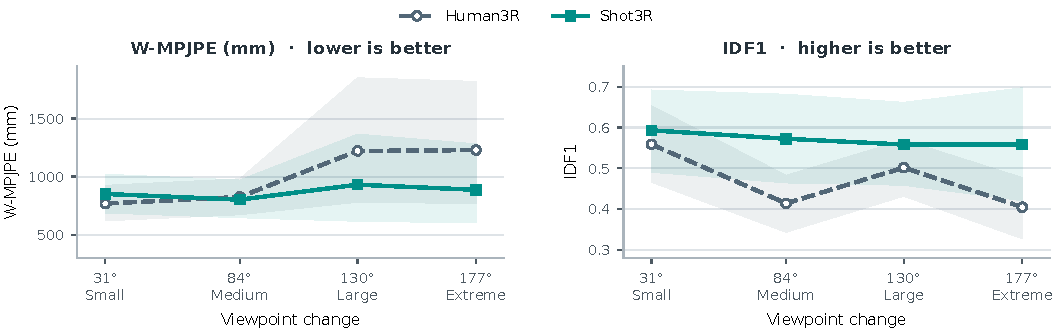
\includegraphics[width=0.82\textwidth]{figures/egohumans_angle_strata.pdf}
  % 中文图注：EgoHumans 中随镜头视角变化的重建和身份表现。曲线给出四个固定视角区间内的
  % W-MPJPE 和 IDF1 绝对值，阴影为以 capture 为单位 bootstrap 得到的 95% 置信区间。
  % Shot3R 在全部区间均获得更高 IDF1，并在 130° 与 177° 的大视角区间明显降低 W-MPJPE。
  \caption{\textbf{Viewpoint response on EgoHumans.} Curves report absolute
  W-MPJPE and IDF1 in four fixed angle strata; bands are capture-bootstrap 95\%
  confidence intervals. \method{} improves IDF1 throughout, with the clearest
  W-MPJPE reductions at $130^\circ$ and $177^\circ$.}
  \label{fig:angle-strata}
\end{figure*}


% 中文段落标题：与公开方法比较。
% 中文：在双方均可评测的输入上，Shot3R相对OnlineHMR具有更低的人体和相机误差，并在全部序列上取得更高IDF1与Coverage；除EgoHumans WA外，配对区间均不跨零。
% 在Shot3R与JOSH共同可评测的样本上，三个数据集的W/WA/ATE均由Shot3R取得更低结果。TRACE与PromptHMR仅能在22/35和64/87段EgoBody序列上返回可评测W/WA，因此需结合有效样本数理解其条件误差；完整结果见附录。
\paragraph{Comparison with public methods.}
Against OnlineHMR on shared valid inputs, \method{} lowers human and camera
errors and, over all streams, raises IDF1/Coverage; paired intervals exclude
zero except for EgoHumans WA. On streams evaluable by both methods, it also
lowers W/WA/ATE versus the offline JOSH pipeline across all three datasets,
without future-frame access. TRACE and PromptHMR return EgoBody W/WA for only
22/35 and 64/87 streams; Appendix~\ref{app:full-results} reports common
support, paired intervals, failures, and complete metrics.

% 中文小节标题：分析与消融
\subsection{Analysis and Ablation Studies}
\label{sec:ablation}

% 中文段落标题：镜头间对齐与状态传播。
% 中文：只重置状态会失去跨镜头世界坐标联系。随后使用同一原版Human3R权重、相同切换后RGB和静态物理相机，
% 比较状态延续与重新初始化；首帧锚定消除固定坐标偏移，且两种控制都不使用Shot3R模块。
\paragraph{Alignment and state propagation.}
Reinitialization alone loses the inter-shot reference, increasing EgoBody
W/WA from 321.1/233.4 to 752.6/589.4\,mm. To isolate state interference, we use
the same original \humanthree{} checkpoint on identical post-transition frames
in 90 EgoHumans cases with a static physical camera and no \method{} module.
Both trajectories are anchored to their first new-shot prediction, removing
any fixed coordinate transform. Over the next 16 frames, continuation produces
1.124\,m/$14.58^\circ$ camera drift, versus 0.026\,m/$0.20^\circ$ after
reinitialization, with the latter lower on all 27 captures. Paired mean
differences are 1.098\,m [0.832, 1.372] and
$14.38^\circ$ [$8.92^\circ$, $20.49^\circ$], with
$p=7.45\!\times\!10^{-9}$ for both one-sided paired tests. The preceding state
therefore induces time-varying within-shot error, not merely a fixed coordinate
offset; full statistics are in Appendix~\ref{app:egohumans-state-isolation}.

\begin{figure*}[t]
  \centering
  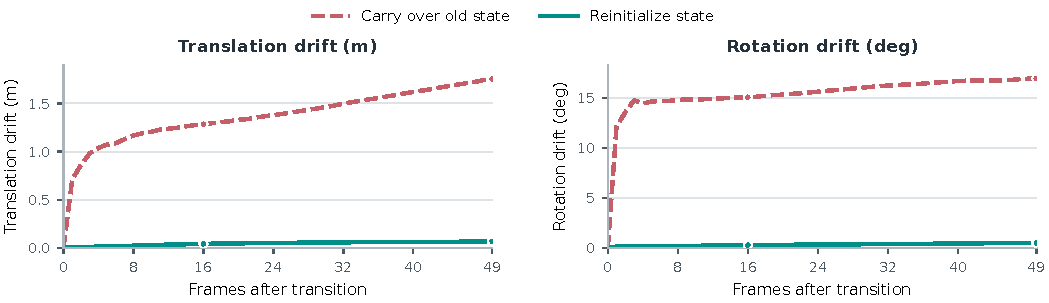
\includegraphics[width=0.80\textwidth]{figures/state_carryover_drift.pdf}
  % 中文图注：静态相机采集上的旧状态延续控制。相同的未修改Human3R权重处理相同的新镜头RGB，不使用Shot3R模块；
  % 首帧锚定消除固定坐标变换。旧状态延续产生镜头内漂移，而重新初始化保持稳定。
  \caption{\textbf{Old-state carry-over causes within-shot camera drift.}
  On static-camera captures, the same unmodified \humanthree{} checkpoint
  processes identical new-shot RGB with no \method{} module. First-prediction
  anchoring removes any fixed transform; carry-over then drifts while
  reinitialization remains stable.}
  \label{fig:state-drift}
\end{figure*}

\begin{table*}[t]
  \centering
  % 中文图注：EgoBody 上的对齐—状态传播 2×2 受控实验及完整 Shot3R。
  % 执行边界操作的三个受控设置使用标注镜头边界，Human3R 不读取边界，完整 Shot3R 使用在线检测边界。
  \caption{Alignment--state-propagation $2\!\times\!2$ control and the complete
  \method{} on EgoBody.}
  \label{tab:mechanism-evidence}
  \scriptsize
  \setlength{\tabcolsep}{2.0pt}
  % 中文列名：设置；边界信号；历史条件对齐；后续传播状态；跨镜头人物关联；
  % W-MPJPE（毫米）；WA-MPJPE（毫米）；ATE（米）；IDF1。
  \resizebox{\textwidth}{!}{%
  \begin{tabular}{lccccrrrr}
    \toprule
    \multirow{2}{*}{Configuration} & \multirow{2}{*}{Boundary cue} &
    \multicolumn{3}{c}{Shot-transition operation} &
    \multicolumn{4}{c}{EgoBody metrics} \\
    \cmidrule(lr){3-5}\cmidrule(lr){6-9}
    & & Alignment & \shortstack{Propagated\\state} & Association &
    W (mm) $\downarrow$ & WA (mm) $\downarrow$ & ATE (m) $\downarrow$ & IDF1 $\uparrow$ \\
    \midrule
    \humanthree{} & --- & \xmark & Continued & \xmark &
      321.1 & 233.4 & 0.124 & 0.870 \\
    State reinitialization & Annotated & \xmark & Reinitialized & \xmark &
      752.6 & 589.4 & 1.141 & 0.834 \\
    Alignment + continued state & Annotated & \cmark & Continued & \xmark &
      293.3 & 227.3 & 0.082 & 0.868 \\
    \shortstack[l]{Alignment +\\reinitialized state} & Annotated & \cmark & Reinitialized & \xmark &
      352.8 & 267.7 & 0.017 & 0.834 \\
    \textbf{\method{}} & Detected & \cmark & Reinitialized & \cmark &
      \textbf{258.8} & \textbf{201.7} & \textbf{0.016} & \textbf{0.985} \\
    \bottomrule
  \end{tabular}%
  }
  \vspace{1pt}

  % 中文表下注释：标注边界用于三个执行边界操作的受控设置；Human3R 不使用边界信号。
  % 两个已对齐设置关闭显式人物关联与人物引导的共享平移，只改变对齐后传播的状态。
  \parbox{0.96\textwidth}{\scriptsize Annotated boundaries are used only by
  the controlled configurations; \humanthree{} receives no boundary cue. The
  two aligned controls disable association and person-guided translation, so
  only the state propagated after alignment changes.}
\end{table*}


% 中文：在相同标注边界和学习式对齐下，两个控制仅改变对齐后传播的状态。延续状态有利于人体世界坐标估计，
% 重新初始化状态则显著降低序列相机漂移，因此两种策略各有代价。完整Shot3R取得最好的联合结果，但该行评估的是完整设计而非单一组件。
Under the same annotated boundary and learned alignment, propagating the
history-conditioned versus reinitialized state gives identical first-frame
alignment error. With association and person-guided translation disabled,
continued state benefits world-frame human estimates (293.3/227.3 versus
352.8/267.7\,mm W/WA), whereas reinitialization improves sequence ATE (0.017
versus 0.082\,m); the 43-recording paired ATE difference is 0.065\,m
[0.049, 0.085]. Thus neither state choice is uniformly better. The complete
system combines reinitialized recurrence, association, and the shared
transform, reaching 258.8/201.7\,mm W/WA, 0.016\,m ATE, and 0.985 IDF1---the
best joint outcome in Table~\ref{tab:mechanism-evidence}. Because this row
evaluates the combined design, its gains are not attributed to state choice
alone. Together, the controls support treating alignment and recurrent-state
propagation as separate decisions.

% 中文段落标题：人物关联。
% 中文：Harmony4D中，骨盆位置已提供有效关联；依次加入躯干朝向与关节结构会进一步提高延续率和IDF1，说明三种预测几何线索互补。
\paragraph{Person association.}
On Harmony4D, pelvis position already provides effective association.
Augmenting it with torso orientation and root-centered joints raises identity
continuation from 78.41\% to 80.68\% and IDF1 from 0.620 to 0.635, supporting
the complementarity of the predicted geometric cues. Complete denominators
and results are reported in Appendix~\ref{app:harmony-association}; association
remains a lightweight supporting mechanism after inter-shot alignment.

% 中文段落标题：重复镜头切换。
% 中文：补充材料中的小规模三镜头受控实验检验同一状态转换能否重复执行，并完整保留相应的指标权衡。
\paragraph{Repeated shot transitions.}
A small three-shot control in the supplement verifies that the same transition
operation can be reapplied, while retaining the associated metric trade-offs
(Appendix~\ref{app:multicut}).

% 中文段落标题：镜头检测与效率。
% 中文：标准化重建计时包含模型推理、输出解码、人物关联和世界坐标配准，不包含模型加载、图像读取缩放或自动镜头检测。Shot3R一次切换时达到3.106 FPS，而Human3R为3.224 FPS，仅增加3.8%的时间开销。完整系统计时留在补充材料。
\paragraph{Transition detection and efficiency.}
The detector's first trigger matches the annotated transition in every primary
protocol stream. Under the standardized reconstruction protocol, timing
includes model inference, output decoding, person association, and
world-coordinate registration, but excludes model loading, RGB loading and
resizing, and automatic transition detection. On one NVIDIA L20, \method{}
with one transition processes 100 frames at 3.106 FPS, compared with 3.224 FPS
for \humanthree{}, corresponding to 3.8\% additional time. A transition adds
one neural evaluation at its first frame. Appendix~\ref{app:implementation}
reports the controlled breakdown, transition-count study, and separate
full-system timing for all seven methods.
